\documentclass{article}

\usepackage[pdftex]{graphicx}
\usepackage[czech]{babel}
\usepackage[utf8]{inputenc}
\usepackage{enumitem}
\usepackage{amsmath}
\usepackage{url}
\usepackage{listings}
\usepackage{caption}
\usepackage[usenames,dvipsnames,svgnames,table]{xcolor}
\usepackage{lstlangarm}

\usepackage[pdftex]{hyperref}
\hypersetup{colorlinks=true,
  unicode=true,
  linkcolor=black,
  citecolor=black,
  urlcolor=black,
  bookmarksopen=true}

\usepackage{xcolor}
\colorlet{mygray}{black!30}
\colorlet{mygreen}{green!60!blue}
\colorlet{mymauve}{red!60!blue}
\lstset{
	backgroundcolor=\color{gray!10},  
	basicstyle=\ttfamily,
	columns=fullflexible,
	breakatwhitespace=false,      
	breaklines=true,                
	captionpos=b,                    
	commentstyle=\color{mygreen}, 
	extendedchars=true,              
	frame=single,                   
	keepspaces=true,             
	keywordstyle=\color{blue},      
	language=c++,                 
	numbers=none,                
	numbersep=5pt,                   
	numberstyle=\tiny\color{blue}, 
	rulecolor=\color{mygray},        
	showspaces=false,               
	showtabs=false,                 
	stepnumber=5,                  
	stringstyle=\color{mymauve},    
	tabsize=3,                      
	title=\lstname                
}

\usepackage[numbers,sort&compress]{natbib}

\newcommand*\justify{
  \fontdimen2\font=0.4em
  \fontdimen3\font=0.2em
  \fontdimen4\font=0.1em
  \fontdimen7\font=0.1em
  \hyphenchar\font=`\-
}

\author{Martin Úbl}

\title{KIV/OS - cvičení č. 8}

\begin{document}

\maketitle



\section{Obsah cvičení}

\begin{itemize}
	\item stránkování, higher-half kernel, ochrana paměti, TLB
	\item izolace uživatelských procesů, crt0
	\item terminate, yield, data a prefetch abort
\end{itemize}

\section{Ochrana paměti na ARM}

Ze základní sady mechanismů ochrany paměti obsahuje ARM procesor obsažený v BCM2835 pouze stránkování. Segmentace zde přítomna není, byť je v embedded světě poměrně hojně zastoupena v určitých odvětvích (v určité redukované podobě). Z pokročilých metod ochrany obsahuje ARM např. TrustZone technologii, ale tu zde probírat nebudeme.

Celý mechanismus stránkování je pochopitelně poměrně rozsáhlý a my si probereme jen nutnou část, kterou budeme potřebovat pro ochranu paměti (ve smyslu izolace uživatelských procesů, i ve smyslu přístupových práv pro spouštění, čtení a psaní do určitých regionů) a pro zvýšení výkonu (TLB, cache, buffering, apod.).

Tento ARM podporuje dvouúrovňovou hierarchii tabulek stránek s tím, že dovoluje mít zavedené až dvě hierarchie v jeden čas. V registrech \texttt{ttbr0} a \texttt{ttbr1} (zkr. \emph{Translation Table Base Register}) se nachází fyzická adresa tabulky stránek, která je momentálně používána. Registr \texttt{ttbr0} se používá pro dolní část adresního prostoru, \texttt{ttbr1} pak pro horní část. Hranice mezi \uv{dolní} a \uv{horní} částí se nachází na místě definovaném v \emph{boundary} fieldu v jednom z registrů, o kterých budeme ještě mluvit -- pro teď lze prozradit to, že tuto hranici posuneme co nejvýše to jde, čímž vyřadíme registr \texttt{ttbr1} ze hry a budeme fakticky používat jen \texttt{ttbr0}, který se bude starat o překlady celého adresního prostoru.

Prakticky se pak adresní prostor dělí kvůli tomu, aby mohl registr \texttt{ttbr0} být střídán dle aktuálně zavedeného uživatelského procesu (a spravoval adresní prostor procesu), a registr \texttt{ttbr1} vždy ukazoval na tabulku stránek jádra (a tedy jsme nemuseli vždy kopírovat mapování jádra do všech tabulek stránek). Pro jednoduchost a z důvodu úspory času však tento princip vynecháme, byť je žádoucí ho pro praktické použití využít.

Dvouúrovňová struktura tabulek stránek dovoluje dělit adresní prostor v první úrovni na bloky o velikosti 1MB, a ve druhé úrovni až na bloky o velikosti 4kB. Podobně jako na jiných architekturách, tak i zde je možnost využít třeba jen první úroveň, a mít tedy stránky o velikosti 1MB. To pochopitelně nemusí být praktické, jelikož se vždy za každých okolností alokují násobky 1MB, a jelikož potřebujeme mít oddělené procesy od jádra a od sebe navzájem, znamenalo by to, že pro jeden proces vždy alokujeme alespoň 2MB (jedna stránka pro kód + data a jedna pro zásobník), byť sám o sobě může vyžadovat jen jednotky kilobajtů. My pro teď však ponecháme dělení pouze na první úroveň, jelikož je to pro nás jednodušší, principy stránkování a ochrany paměti to demonstruje dostatečně a RPi Zero má 512 MB RAM, takže se nám nejspíš paměť vyčerpat nepovede. \textbf{Ovšem,} prakticky, chceme dělit stránky drobněji, pokud to náš use-case vyžaduje (což často např. u interaktivních systémů vyžaduje).

\subsection{System control coprocessor}

Stránkování zajišťuje jednotka správy paměti (Memory Management Unit, MMU), kterou \uv{ovládá} koprocesor zvaný \emph{system control coprocessor} (z praktických důvodů nepřekládáno).

V prvních cvičeních jsme zmínili, že kromě základní sady registrů má ARM procesor ještě další, částečně skryté. \uv{Částečně} proto, že nemají konkrétní mnemonický přepis a nelze k nim přistupovat přímo (např. \texttt{mov r0, \#96}). Namísto toho je potřeba si jejich obsah přesouvat pomocí obecných registrů a instrukcí \texttt{mcr} a \texttt{mrc} (neplést s \texttt{msr} a \texttt{mrs}, ty jsou mj. pro manipulaci s registrem \texttt{cpsr}).

Instrukce \texttt{mcr} a \texttt{msr} má následující podobu:
\begin{lstlisting}
mcr <coprocessor>, <opcode1>, <Rt>, <CRn>, <CRm>[, <opcode2>]
msr <coprocessor>, <opcode1>, <Rt>, <CRn>, <CRm>[, <opcode2>]
\end{lstlisting}
Zde \texttt{coprocessor} označuje konkrétní koprocesor, jehož registry vyžadujeme, \texttt{opcode1} pak jakousi skupinu registrů dle účelu, \texttt{Rt} je obecný registr, jehož obsah bude buď nahrazen obsahem daného koprocesorového registru (\texttt{mrc}) nebo naopak (\texttt{mcr}). \texttt{CRn} a \texttt{CRm} jsou pak číselné lokátory registrů, které lze vyčíst z dokumentace k procesoru. Volitelně pak můžeme uvést \texttt{opcode2}, pokud je hierarchie registrů složitější.

Seznam registrů, jejich opkódy a lokátory lze nalézt například zde: \url{https://developer.arm.com/documentation/ddi0301/h/system-control-coprocessor/system-control-processor-registers/register-allocation?lang=en}

Pro nás budou zajímavé zejména:
\begin{description}
	\item[c1, Control Register] -- zde budeme zapínat cache, MMU a jiné
	\item[c1, Auxiliary Control Register] -- další nastavení cache
	\item[c2, Translation Table Base Register 0 a 1] -- již zmíněné \texttt{ttbr0} a \texttt{ttbr1} registry
	\item[c2, Translation Table Base Control Register] -- zde budeme nastavovat boundary
	\item[c3, Domain Access Control] -- zde zapneme paměťovou doménu
	\item[c7, c8] -- odtud budeme potřebovat zejména registry pro vyprázdnění TLB a invalidaci cache
\end{description}

Například když budeme chtít nahrát nový obsah registru \texttt{ttbr0} (třeba z registru \texttt{r4}), můžeme použít následující instrukci:
\begin{lstlisting}
mcr p15, 0, r4, c2, c0, 0
\end{lstlisting}

\subsection{Paměťová mapa (nová)}

Zavedení ochrany paměti, které jde ruku v ruce s principem izolace procesů, nutně vyžaduje změny v paměťové mapě. 

Především každý proces musí být zaveden (a samozřejmě již při překladu relokován) na jednotnou adresu, a zároveň musí mít iluzi toho, že je v paměti \uv{sám}. Fyzicky pochopitelně bude na adrese, která zrovna byla jádrem vyhrazená v momentě zavedení procesu. Stejně tak bude ve fyzické paměti reálně sedět vedle procesů ostatních. Tím, že pro každý proces vytvoříme tabulku stránek, jsme schopni procesům dodat představu o podobě adresního prostoru, jakou zrovna potřebujeme.

Původní paměťový layout vypadal zhruba jako na obrázku \ref{obr:oldmem}. Doteď jsme uvažovali, že každý proces běží ve stejném adresním prostoru, a tedy je relokován na místo, které mu bylo přiděleno již při překladu jádra. Tato varianta je u systémů reálného času také možná a pro vybrané aplikace i preferovaná kvůli jednoduchosti. Stránkování totiž pochopitelně přináší kromě výhod i nevýhody -- jednou z nich je jistá přidaná režie a tedy ztráta na výkonu.

\begin{figure}[ht!]
	\centering
	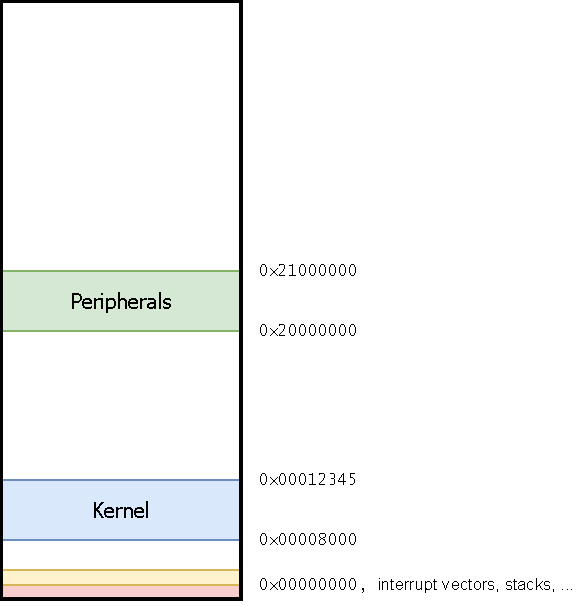
\includegraphics[width=0.5\textwidth]{memmap_old.pdf}
	\caption{Paměťová mapa (virtuální adresní prostor) před stránkováním a izolací procesů}\label{obr:oldmem}
\end{figure}

\begin{figure}[ht!]
	\centering
	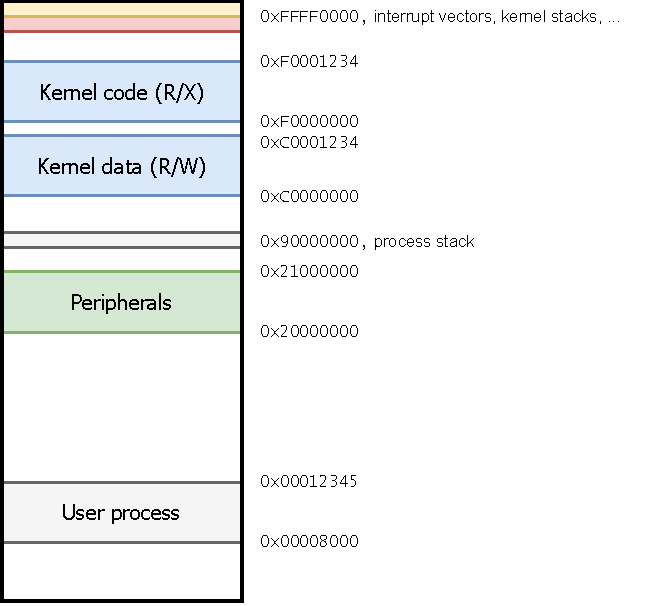
\includegraphics[width=0.5\textwidth]{memmap_new.pdf}
	\caption{Paměťová mapa (virtuální adresní prostor) připravená pro stránkování a izolaci procesů}\label{obr:newmem}
\end{figure}

Nově tedy vyžadujeme, aby byl každý proces zavedený na stejné adrese. Abychom dodrželi relokaci se současným stavem, ponechme začátek rovněž na adrese \texttt{0x8000}. Zároveň ale nějak potřebujeme volat služby jádra pomocí systémových volání -- jejich obslužný kód musí být někde zavedený. Jednou možností je mít pro jádro vlastní adresní prostor (tedy později tabulku stránek). To samozřejmě možné je, ale připravíme se o poměrně velkou část výhod cache a TLB -- každé přepnutí tabulky stránek znamená, že veškeré look-ahead operace a cachované look-upy budou ztraceny, protože v novém layoutu nemají smysl. Pro každé systémové volání by se tedy musel vyprázdnit TLB, cache a jiné, a to není zrovna to nejlepší.

Lepším řešením je nechat kód a data jádra v paměťovém prostoru každého procesu, a systémové volání využít jen na to, abychom změnili úroveň oprávnění a začali vykonávat vstupní bod jádra. Pochopitelně nemůžeme nechat kód jádra nechráněný -- jeho spouštění podmíníme privilegovaným režimem, což později rovněž dovolí samotný mechanismus stránkování.

Stejně tak je dobré se zbavit obsazených spodních adres, kam jsme umístili tabulku vektorů přerušení a zásobníky jádra. Díky koprocesoru je možné tabulku vektorů přerušení relokovat do horní části adresního rozsahu (adresa {\tt 0xFFFF0000} - {\tt 0xFFFF001C}). Zásobníky si pak přemístíme ručně v inicializačním kódu jádra. Dále bude zásobník potřebovat i každý proces. Namapujme ho na nějakou námi zvolenou adresu, třeba {\tt 0x90000000}. Zásobník by měl být opět umístěn na stejnou adresu, která je dobře známá -- OS pak nastaví procesový stack pointer na vrchol zásobníku, který bude pro každý proces na stejné virtuální adrese. Nový paměťový layout tedy lze vidět na obrázku \ref{obr:newmem}.

\subsubsection{Higher-half kernel}

Výše jsme zmínili, že umístíme kernel data a kód do horní části adresního rozsahu, tedy na místo, kde nám \uv{nevadí} a je systematicky využitelný např. při systémových voláních. Tento způsob relokace jádra se obecně nazývá \emph{kernel in higher-half}, popř. jen \emph{higher-half kernel} (někdy \emph{upper-half}).

K tomu, aby kernel mohl běžet na vyšších adresách, nutně potřebujeme stránkování. Ovšem vyvstává problém -- kde bude kód, který zapne stránkování, a jak se vlastně do \emph{higher-half} dostaneme?

My technicky vzato nepotřebujeme mít relokovanou celou kernelovou paměť. Stačí nám pouze takový kus, který bude využívaný v dalším běhu systému. S trochou fantazie jde tato množina dat a kódů minimalizovat, ale pro nás bude bohatě dostačovat, když relokujeme do horních adres celý náš dosavadní kernel, a \uv{dole} (na původní adrese {\tt 0x8000}) necháme jen kritický kód, který je potřeba k inicializaci stránkování.

\subsection{TLB, cache a predikce skoků}

ARM procesory ve většině provedení podporují v souvislosti s mechanismem stránkování i TLB, instrukční a datovou cache a další.

Instrukční a datová cache je oddělená a je potřeba ji zapnout. Explicitně lze ovládat vybrané parametry cachování, pro nás bude teď stačit obě cache zapnout příslušnými příznaky v MMUCR registru. Rovněž v MMUCR registru objevíme příznak pro zapnutí predikce skoků. Všechny tyto principy jsou velice důležitým nástrojem při optimalizacích běhu. Moderní systémy, které cílí na výkon, se bez predikce skoků a takto uspořádaných cache v podstatě neobejdou.

Jakýmsi doplňkovým mechanismem je pak \emph{Translation Look-aside Buffer} (TLB). To je relativně malé asociativní úložiště pro cachování výsledků překladu virtuální adresy na adresu fyzickou (stránkování). Procesor obsažený v RPi Zero obsahuje dvě tzv. MicroTLB (jedna pro prefetch (instrukce), jedna pro data) o velikosti 10 záznamů, a jednu hlavní TLB o velikosti 64 záznamů. MicroTLB má znatelně kratší dobu přístupu, jelikož je takto malá a plně asociativní.

TLB budeme vždy potřebovat řádně vyprázdnit (invalidovat), když budeme měnit tabulky stránek. ARM je na tohle ale tak trochu připravený -- podobně jako u jiných architektur existuje ASID (Application-Specific ID) nebo jeho obdoba, tak ARM dovoluje překlady adres dělit do tzv. domén. Těch definuje celkem 16 a je čistě na implementátorovi, zda nějaké použije, a pokud ano, tak jaké.

S doménovým dělením dělat nebudeme, jelikož to vyžaduje trochu kódu a logiky navíc. Ponechme vše v jedné doméně a TLB vždy invalidujme. Důležité je vědět, že takový mechanismus existuje, protože dovede běh systému zefektivnit.

\section{Stránkování a inicializace jádra}

Nejdříve musíme někam umístit kód, který stránkování inicializuje. Vytvořme novou sekci \texttt{.initsys} pro kód a \texttt{.initsys.data} pro data, kam vložíme kód a data relevantní k inicializaci stránkování. Sekce \texttt{.initsys} a \texttt{.initsys.data} budou relokovány na původní adresu kódu a dat, tedy na adresu \texttt{0x8000}. Projistotu vytvoříme i sekci \texttt{.initsys.start} pro vstupní bod jádra. Kód této sekce se spustí pouze jednou, na začátku zavádění systému.

\subsection{Linker skript}

Upravme linker skript, aby zohledňoval \texttt{initsys} sekce, relokoval kód jádra na \texttt{0xF0000000}, data jádra na \texttt{0xC0000000}, a definoval symboly tak, abychom je mohly z kódu vyzvednout:
\begin{lstlisting}
ENTRY(_start)

MEMORY
{
	initsys_base : ORIGIN = 0x8000, LENGTH = 0x10000
	kernel : ORIGIN = 0xF0000000, LENGTH = 0x100000
	kerneldata : ORIGIN = 0xC0000000, LENGTH = 0x100000
}

SECTIONS
{
	.initsys :
	{
		*(.initsys.start*)
		*(.initsys*)
	} > initsys_base
	
	.initsys.data :
	{
		*(.initsys.data*)
	} > initsys_base
	
	__kernel_high_code = ALIGN(4k);
	_virt_code_start = 0xF0000000;

	.text (__kernel_high_code + _virt_code_start) : AT(__kernel_high_code)
	{
		*(.text*)
	} > kernel
	
	.rodata : {
		*(.rodata*)
	} > kernel
	
	_virt_code_end = ABSOLUTE(.);
	__high_data_start = ALIGN(4k);
	
	_virt_data_start = 0xC0000000;
	
	.data (_virt_data_start + __high_data_start - _virt_code_start) : AT(__high_data_start - _virt_code_start)
	{
		__CTOR_LIST__ = .; *(.ctors) *(.init_array) __CTOR_END__ = .; 
		__DTOR_LIST__ = .; *(.dtors) *(.fini_array) __DTOR_END__ = .;
		data = .;
		_data = .;
		__data = .;
		*(.data)
		
	} > kerneldata
	
	_virt_bss_start = .;
	
	.bss :
	{
		*(.bss*)
		*(COMMON)
	} > kerneldata
	
	_virt_bss_end = .;
	_virt_data_end = ALIGN(4k);

	_phys_code_start = 0x00000000;
	_phys_code_end = _phys_code_start + (_virt_code_end - _virt_code_start);

	_phys_data_start = __high_data_start - _virt_code_start;
	_phys_data_end = _phys_data_start + (_virt_data_end - _virt_data_start);

	_phys_bss_start = _phys_data_start + (_virt_bss_start - _virt_data_start);
	_phys_bss_end = _phys_data_start + (_virt_bss_end - _virt_data_start);
}
\end{lstlisting}
Zde mimo jiné můžeme vidět různá zarovnání a posuny, a to tak, aby vždy sekce začínala zarovnaná vzhledem k rámcům paměti (stránkám). Nyní můžeme začít psát příslušný kód.

% initsys sekce
% link.ld
% priprava zasobniku
% tabulka vektoru preruseni

\subsection{Inicializace systému}

Nejprve naplníme tabulku vektorů přerušení, a to stejně jako doteď, jen se připravme na její relokaci do vyšších adres. Výše jsme zmínili, že lze zapnutím příznaku v řídicím registru donutit systém, aby tuto tabulku hledal na adrese {\tt 0xFFFF0000}. Pokud uvážíme, že stránky budou o velikosti 1 MiB ({\tt 0x00100000}) a my musíme provést mapování celé stránky, tak nejbližší nižší násobek je {\tt 0xFFF00000} (tedy tato stránka bude mít rozsah od {\tt 0xFFF00000} do {\tt 0xFFFFFFFF}), a fakticky se tedy jedná o stránku poslední. Tabulku vektorů přerušení tedy budeme kopírovat ne na fyzickou adresu {\tt 0x0}, ale {\tt 0xF0000}, protože pak můžeme namapovat celý první rámec na poslední, a tabulka vektorů přerušení se objeví tam, kde ji potřebujeme mít. Nutně to ale znamená, že dokud nezapneme stránkování, nebudou nám fungovat přerušení. To ale nevadí -- ani to nemáme v úmyslu.

Poté potřebujeme inicializovat zásobník, a to stejně, jako jsme to dělali doteď -- jen je to dočasné do doby, než se přepneme do nového adresního prostoru. Tam toto nastavení provedeme znovu, jen na adresy v horní části adresního rozsahu. Rovněž proveďme nulování {\tt .bss} sekce -- čím dříve, tím lépe.

Nastavíme tedy tabulku vektorů přerušení, zásobníky, vynulujeme {\tt .bss} sekci a skočíme do kódu v jazyce C (např. funkce {\tt \_init\_system\_memory}, kterou vytvoříme později), který bude provádět zbytek (stránkování). Kód sekce {\tt .initsys} a {\tt .initsys.start} v souboru {\tt start.s} bude vypadat tedy nějak takto:
\begin{lstlisting}
.section .initsys.start

.global _start

_start:
    ldr pc, _reset_ptr
    ldr pc, _undefined_instruction_ptr
    ;@ ...    
    ;@ ... zredukovano, kod je shodny jako doted ...

_reset:
    mov r0, #0x8000
    mov r1, #0xF0000        ;@ nove adresa 0xF0000

    ldmia r0!,{r2, r3, r4, r5, r6, r7, r8, r9}
    stmia r1!,{r2, r3, r4, r5, r6, r7, r8, r9}
    ldmia r0!,{r2, r3, r4, r5, r6, r7, r8, r9}
    stmia r1!,{r2, r3, r4, r5, r6, r7, r8, r9}

    mov r4, #0x00000000

    ;@ vyuzivame ted jen SYS mod, pozdeji nastavime zbytek
    mov r0, #(CPSR_MODE_SYS | CPSR_IRQ_INHIBIT | CPSR_FIQ_INHIBIT)
    msr cpsr_c, r0
    add sp, r4, #0x4000

    ;@ C startup kod (nulovani .bss sekce)
    bl _c_startup
    bl _init_system_memory
init_hang:
    b init_hang
\end{lstlisting}

Tento kód provede nutnou část v assembly, kterou mj. potřebujeme k tomu, abychom vůbec mohli volat funkce. Pak vytvořme soubor {\tt initsys.cpp}, kde budeme s inicializací pokračovat.

Funkce a proměnné (konstanty) v tomto souboru budeme nyní dekorovat atributy dle jejich sekcí, aby bylo explicitně jasné, kde se nachází. Nutno dodat, že kód budeme ukládat do sekce {\tt .initsys} (resp. {\tt .text}) a proměnné (konstanty) do sekce {\tt .initsys.data} (resp. {\tt .data}). Tento atribut je potenciálně závislý na překladači, pro gcc je to:

\begin{lstlisting}
__attribute__((section("nazevsekce")))
\end{lstlisting}

Na příkladu funkce a proměnné relokovaných do {\tt .initsys} a {\tt .initsys.data} sekcí:
\begin{lstlisting}
int __attribute__((section(".initsys"))) moje_funkce() {
    // ...
}

__attribute__((section(".initsys.data"))) uint32_t moje_promenna;
\end{lstlisting}

Do tohoto souboru přesuňme funkci {\tt \_c\_startup}, kterou jsme nejspíše definovali jinde. Tady je navíc potřeba ji dekorovat atributem sekce, jelikož ji budeme potřebovat v dolní části rozsahu.

\subsection{Tabulka stránek}

Dále budeme pokračovat nastavením tabulky stránek. Předtím, než tak začneme činit, si stáhněte definice příznaků a polí z tohoto odkazu: \url{https://home.zcu.cz/~ublm/files/os/mmuflags.h}. Obsah tohoto souboru si volně začleňte do svého projektu.

Nyní vytvořme tabulku stránek v dolní části rozsahu (později ji budeme adresovat jinak) -- zarovnáme ji na velikost rámce a relokujeme do patřičné sekce. Velikost tabulky je implementačně pevně daná na 4096 záznamů, každý záznam identifikuje adresní rozsah o pevně dané velikosti (1 MiB):
\begin{lstlisting}
constexpr uint32_t PT_Size = 4096;

constexpr uint32_t PT_Region_Size = 0x100000;
	
volatile __attribute__ ((aligned (0x4000))) __attribute__((section(".initsys.data"))) uint32_t Page_Directory_Kernel[PT_Size];
\end{lstlisting}

Definujme ještě pomocnou funkci pro \uv{překlad} virtuální adresy na index v tabulce stránek -- jelikož krokujeme po 1 MiB (velikost rámce a stránky v 1. úrovni), stačí tuto funkci definovat jako prostý posun:
\begin{lstlisting}
static uint32_t __attribute__((section(".initsys"))) PT_Entry(uint32_t addr) {
	return addr >> 20;
}
\end{lstlisting}

Vytvořme dále funkci {\tt \_init\_system\_memory}, kterou se snažíme volat z kódu v assembly. Povšimněte si dekorace atributem \texttt{noreturn} -- my se z této funkce vlastně nebudeme vracet, budeme se přesouvat do vrchní části adresního rozsahu jiným způsobem, který zásobník obchází a navíc ho tamější kód okamžitě vyprázdní:
\begin{lstlisting}
extern "C" void __attribute__((section(".initsys"))) __attribute__((noreturn)) _init_system_memory() {
	// ...
\end{lstlisting}

Sem budeme nyní dopisovat inicializační kód stránkování.

Jako první tabulku vyprázdníme -- do každého prvku tabulky vložíme spodní bity, které označují neplatný záznam (který vyústí v abort):
\begin{lstlisting}
for (uint32_t i = 0; i < PT_Size; i++) {
    Page_Directory_Kernel[i]
          = DL1_Flags::Access_Type_Translation_Fault;
}
\end{lstlisting}

Co teď? Potřebujeme do výchozí (pro teď prostě \emph{kernelové}) tabulky stránek dostat několik regionů, z nichž některé budou jen dočasné:
\begin{enumerate}
	\item {\tt 0x00000000}-{\tt 0x1FFFFFFF} na {\tt 0x00000000}-{\tt 0x1FFFFFFF} (dočasně) - dočasně zavedeme tzv. \emph{identity mapping} na spodní část rozsahu, a to proto, aby nedošlo k výpadku stránky v momentě, kdy načteme novou tabulku stránek a zapneme stránkování. Kód, který tohle udělá, se totiž musí nacházet v dolní části rozsahu a neexistuje způsob, jak poté skočit do higher-half bez instrukce, která se nachází stále ještě v dolní části
	\item {\tt 0x20000000}-{\tt 0x20100000} na {\tt 0x20000000}-{\tt 0x20100000} (trvale) - \emph{identity mapping} pro periferie, nastavíme však příznak, aby mohl přistupovat jen privilegovaný režim
	\item {\tt 0xC0000000}-{\tt 0xCFFFFFFF} na {\tt 0x00000000}-{\tt 0x0FFFFFFF} (trvale) - pro kernelová data, resp. v našem případě pro \uv{kernelový pohled} na paměť
	\item {\tt 0xF0000000}-{\tt 0xF1000000} na {\tt 0x00000000}-{\tt 0x01000000} (trvale) - pro kernelový kód
	\item {\tt 0xFFF00000}-{\tt 0xFFFFFFFF} na {\tt 0x00000000}-{\tt 0x000FFFFF} (trvale) - pro tabulku vektorů přerušení a systémové zásobníky
\end{enumerate}

Jak je vidět, téměř všechna z těchto mapování je jen jiný pohled na fyzickou paměť. Pro to máme v adresním prostoru spousty místa, alespoň v případě RPi Zero -- fyzické paměti máme 512 MiB, ale adresovat jsme schopni až 4 GiB. To znamená, že fyzická paměť zabírá jen osminu adresního prostoru. Kdyby tomu tak nebylo, a fyzické paměti bychom měli více, tak musíme být pochopitelně daleko kreativnější v mapování esenciálních dat a kódu, který je pro běh kritický.

Pro dané regiony bude platit následující (číslo odpovídá odrážce v předchozím seznamu):
\begin{enumerate}
	\item pro čtení, zápis i spouštění, jen pro privilegovaný režim (i když na úrovni oprávnění moc nezáleží)
	\item čtení a zápis v privilegovaném režimu, zakážeme cachování a bufferování (aby se zápis i čtení vždy provedlo v momentě, kdy o to žádáme)
	\item čtení a zápis v privilegovaném režimu, zakážeme spouštění (execute)
	\item čtení a zápis v privilegovaném režimu
	\item čtení a zápis v privilegovaném režimu
\end{enumerate}

Pokusme se tedy tabulku stránek naplnit. Všechny záznamy, které vyplňujeme, budou pouze v první úrovni (1 MiB stránky) a budou v doméně 0 -- všechny budou mít příznak \texttt{DL1\_Flags::Access\_Type\_Section\_Address} a \texttt{DL1\_Flags::Domain\_0}. Rovněž uvedeme příznak \texttt{DL1\_Flags::Shareable} -- označuje sdílenou paměť mezi procesory (a jednotkami). Dále budeme přidělovat příznaky "type extension" tak, aby se nám v kombinaci s příznaky pro bufferovatelnost a cachovatelnost povedlo docílit konzistentního provádění/čtení/zápisu. Tyto příznaky různě mění politiku při bufferování a cachování -- více viz \url{https://developer.arm.com/documentation/ddi0301/h/memory-management-unit/memory-region-attributes/c-and-b-bit--and-type-extension-field-encodings?lang=en}.

Pro bod 1 (dočasný identity mapping):
\begin{lstlisting}
for (addr = 0;
     addr < 0x20000000;
     addr += PT_Region_Size)
{
    Page_Directory_Kernel[PT_Entry(addr)] = addr
        | DL1_Flags::Access_Type_Section_Address
        | DL1_Flags::Bufferable
        | DL1_Flags::Cacheable
        | DL1_Flags::Domain_0
        | DL1_Flags::Access_Privileged_RW_User_None
        | DL1_Flags::TEX_001
        | DL1_Flags::Shareable;
}
\end{lstlisting}

Pro bod 2 (periferie a memory-mapped I/O):
\begin{lstlisting}
for (addr = hal::Peripheral_Base;
     addr < hal::Peripheral_Base + 0x01000000;
     addr += PT_Region_Size)
{
    Page_Directory_Kernel[PT_Entry(addr)] = addr
        | DL1_Flags::Access_Type_Section_Address
        | DL1_Flags::Domain_0
        | DL1_Flags::Access_Privileged_RW_User_None
        | DL1_Flags::TEX_000
        | DL1_Flags::Shareable;
}
\end{lstlisting}

Pro bod 3 (kernel data):
\begin{lstlisting}
for (addr = 0xC0000000;
     addr < 0xD0000000;
     addr += PT_Region_Size)
{
    Page_Directory_Kernel[PT_Entry(addr)] = (addr - 0xC0000000)
        | DL1_Flags::Access_Type_Section_Address
        | DL1_Flags::Cacheable
        | DL1_Flags::Domain_0
        | DL1_Flags::Execute_Never
        | DL1_Flags::Access_Privileged_RW_User_None
        | DL1_Flags::TEX_000
        | DL1_Flags::Shareable;
}
\end{lstlisting}

Pro bod 4 (kernel kód):
\begin{lstlisting}
for (addr = 0xF0000000;
     addr < 0xF1000000;
     addr += PT_Region_Size)
{
    Page_Directory_Kernel[PT_Entry(addr)] = (addr - 0xF0000000)
        | DL1_Flags::Access_Type_Section_Address
        | DL1_Flags::Bufferable
        | DL1_Flags::Cacheable
        | DL1_Flags::Domain_0
        | DL1_Flags::Access_Privileged_RW_User_None
        | DL1_Flags::TEX_001
        | DL1_Flags::Shareable;
}
\end{lstlisting}

Pro bod 5 (tabulka vektorů přerušení a zásobník):
\begin{lstlisting}
Page_Directory_Kernel[PT_Entry(0xFFF00000)] = 0
    | DL1_Flags::Access_Type_Section_Address
    | DL1_Flags::Bufferable
    | DL1_Flags::Cacheable
    | DL1_Flags::Domain_0
    | DL1_Flags::Access_Privileged_RW_User_R
    | DL1_Flags::TEX_000
    | DL1_Flags::Shareable;
\end{lstlisting}

% priprava tabulky stranek

Nyní máme naplněnou tabulku stránek a mělo by stačit pouze nastavit příznaky v koprocesorových (a MMU) registrech a pak se přesunout do higher-half.

Jelikož chceme používat cache, nastavme v auxiliary control registru velikost cache na 16 kiB:
\begin{lstlisting}
unsigned int auxctl_flags;
asm volatile ("mrc p15, 0, %0, c1, c0, 1" : "=r" (auxctl_flags));
auxctl_flags |= AUXCtl_Flags::Cache_Size_16k;
asm volatile ("mcr p15, 0, %0, c1, c0, 1" :: "r" (auxctl_flags));
\end{lstlisting}

Jak bylo zmíněno, používat budeme jen doménu 0. Proto do domain access control registru nastavme doménu 0 do režimu \uv{klient} (v podstatě jediná myslitelná hodnota v běžném režimu -- u TrustZone ještě můžeme být v pozici správce domény):
\begin{lstlisting}
unsigned int domain_access = DACR_Flags::Client << 0;
asm volatile ("mcr p15, 0, %0, c3, c0, 0" :: "r" (domain_access));
\end{lstlisting}

Pak v translation table base control registru nastavíme \uv{boundary} na maximální možnou -- vypneme tak používání druhého bázového registru a vynutíme mapování řešit jen prvním z nich:
\begin{lstlisting}
unsigned int ttbc = TTBC_Flags::Boundary_16k;
asm volatile ("mcr p15, 0, %0, c2, c0, 2" :: "r" (ttbc));
\end{lstlisting}

Nyní už můžeme nastavit translation table base registr na naši tabulku stránek. Tuto hodnotu tvoří mj. i skupina příznaků -- my zapneme atribut \texttt{Inner\_Cacheable}, aby procesor cachoval obsah tabulky a \texttt{Shared}, abychom opět povolili sdílení mezi procesorovými jednotkami:
\begin{lstlisting}
unsigned int ttbr0 = reinterpret_cast<volatile unsigned int>(&Page_Directory_Kernel)
    | TTBR_Flags::Inner_Cacheable
    | TTBR_Flags::Shared;
asm volatile ("mcr p15, 0, %0, c2, c0, 0" :: "r" (ttbr0));
\end{lstlisting}

Posledním krokem před zapnutím stránkování je vyprázdnění prefetch bufferu a invalidace datové cache -- tento krok pak budeme dělat vždy při přepnutí kontextu:
\begin{lstlisting}
asm volatile ("mcr p15, 0, %0, c7, c5,  4" :: "r" (0) : "memory");
asm volatile ("mcr p15, 0, %0, c7, c6,  0" :: "r" (0) : "memory");
\end{lstlisting}

Nakonec můžeme zapnout MMU a nastavit poslední sadu příznaků. Nastavujeme příznaky pro povolení MMU, datové a instrukční cache, predikce skoků, relokace tabulky vektorů přerušení na adresu \texttt{0xFFFF0000} a povolení rozšířeného formátu tabulky stránek (abychom měli např. příznak \uv{execute never} pro datové sekce). Rovněž pro teď zapneme povolení nezarovnaného přístupu do paměti, což je atribut, který se může hodit pro fázi ladění (v produkci se takový přístup vymstí na výkonu):
\begin{lstlisting}
unsigned int mmucr;
asm volatile ("mrc p15,0,%0,c1,c0,0" : "=r" (mmucr));

mmucr = mmucr
    | MMUCR_Flags::MMU_Enable
    | MMUCR_Flags::Data_Cache_Enable
    | MMUCR_Flags::Branch_Prediction_Enable
    | MMUCR_Flags::Instruction_Cache_Enable
    | MMUCR_Flags::High_Exception_Vectors
    | MMUCR_Flags::Unaligned_Memory_Access_Enable
    | MMUCR_Flags::Disable_Subpage_AP;

asm volatile ("mcr p15,0,%0,c1,c0,0" :: "r" (mmucr) : "memory");
\end{lstlisting}

Pokud jsme něco udělali špatně, tak v tomto bodě bude vyvolán data nebo prefetch abort. Pokud ne, provádění pokračuje dál, jen s tím rozdílem, že jsou přístupy překládány jednotkou pro správu paměti (MMU).

Teď jsme připraveni na skok do \emph{higher-half}, kde z můžeme provést zbytek inicializace jádra. Provedeme tedy skok do funkce \texttt{\_init\_system\_memory\_high} -- nebudeme ji však volat jako funkci, ale rovnou do ní skočíme:

\begin{lstlisting}
asm volatile("mov lr, %[_init_system_memory_high]"
   : :
   [_init_system_memory_high] "r" ((unsigned int)&_init_system_memory_high) );
asm volatile("bx lr");
\end{lstlisting}

Jak bylo zmíněno, při těchto skocích budeme obcházet zásobník. Proto si adresu této funkce načteme do registru {\tt lr} a rovnou tam skočíme. Obsah zásobníku bude totiž stejně záhy zahozen v našem kódu inicializace zásobníků v \emph{higher-half}.

Vytvořme nyní soubor \texttt{mmu.cpp} ve složce se zdrojovými soubory v podsložce \texttt{memory}.

Zde můžeme definovat odkazy na symboly, které nám exportuje až linker (a žádáme si o ně v {\tt link.ld}):
\begin{lstlisting}
extern "C"
{
  extern const uint32_t _virt_code_start;
  extern const uint32_t _virt_data_start;

  extern const uint32_t _phys_bss_start;
  extern const uint32_t _phys_bss_end;
  extern const uint32_t _phys_data_start;
  extern const uint32_t _phys_data_end;
}
\end{lstlisting}

Taktéž definujeme zmíněnou funkci \texttt{\_init\_system\_memory\_high}. V té v podstatě jen potřebujeme vynulovat spodní identity mapping paměti (tedy mapování adres {\tt 0x00000000-0x20000000}), invalidovat cache a TLB a skočit na další fázi inicializace (zásobníky). Tady ovšem nemůžeme použít původní adresu tabulky stránek, ke které jsme přistupovali pomocí adres ve spodní části rozsahu -- logicky odebráním mapování dojde ke ztrátě přístupu. Musíme proto k této paměti přistupovat v regionu kernel dat, tedy pomocí adresy v bloku začínajícím {\tt 0xC0000000}. Jelikož mapujeme tuto sekci v podstatě jen s jinou bází, lze si opatřit ukazatel na tabulku stránek např. takto:

\begin{lstlisting}
uint32_t* const Page_Directory_Kernel_High =
     reinterpret_cast<uint32_t*>(_virt_data_start + reinterpret_cast<uint32_t>(&Page_Directory_Kernel));
\end{lstlisting}

Nyní můžeme smazat mapování spodní části:
\begin{lstlisting}
unsigned int addr;
for (addr = 0; addr < 0x20000000; addr += PT_Region_Size)
  Page_Directory_Kernel_High[PT_Entry(addr)] = 0;
\end{lstlisting}

Pro jistotu invalidujeme datovou cache, prefetch buffer a TLB:
\begin{lstlisting}
asm volatile ("mcr p15, 0, %0, c7, c5,  4" :: "r" (0) : "memory");
asm volatile ("mcr p15, 0, %0, c7, c6,  0" :: "r" (0) : "memory");
asm volatile ("mcr p15, 0, %0, c8, c7,  0" :: "r" (0) : "memory");
\end{lstlisting}

Nyní skočíme zpět do assembly (jen higher-half) a inicializujeme zásobníky. Odtud pak můžeme pokračovat ve vykonávání kódu, který již známe. Teď obdobným způsobem jako dříve skočíme do funkce {\tt kernel\_mode\_start}, kterou si za okamžik definujeme:
\begin{lstlisting}
asm volatile("mov lr, %[kernel_mode_start]"
    : :
    [kernel_mode_start] "r" ((unsigned int)&kernel_mode_start) );
asm volatile("bx lr");
\end{lstlisting}

V assembly (např. {\tt start.s}) pak můžeme definovat tuto funkci a provedeme v ní již zmíněnou inicializaci zásobníků. Tento kód je vlastně identický s tím, který jsme používali v minulých cvičeních. Jediný rozdíl je v bázové adrese zásobníků, která je nyní v horní části adresního prostoru:
\begin{lstlisting}
.section .text

.global kernel_mode_start
  kernel_mode_start:

  ldr r4, =#0xFFFF0000

  mov r0, #(CPSR_MODE_SVR | CPSR_IRQ_INHIBIT | CPSR_FIQ_INHIBIT)
  msr cpsr_c, r0
  add sp, r4, #0x8000

  mov r0, #(CPSR_MODE_IRQ | CPSR_IRQ_INHIBIT | CPSR_FIQ_INHIBIT)
  msr cpsr_c, r0
  add sp, r4, #0x7000

  mov r0, #(CPSR_MODE_FIQ | CPSR_IRQ_INHIBIT | CPSR_FIQ_INHIBIT)
  msr cpsr_c, r0
  add sp, r4, #0x6000

  mov r0, #(CPSR_MODE_ABT | CPSR_IRQ_INHIBIT | CPSR_FIQ_INHIBIT)
  msr cpsr_c, r0
  add sp, r4, #0x5000

  mov r0, #(CPSR_MODE_SYS | CPSR_IRQ_INHIBIT | CPSR_FIQ_INHIBIT)
  msr cpsr_c, r0
  add sp, r4, #0x4000

  bl _cpp_startup
  bl _kernel_main
  bl _cpp_shutdown
upper_half_hang:
  b upper_half_hang
\end{lstlisting}

Nyní jsme ve stavu, kdy máme zapnuté stránkování a zavedené jádro do \emph{higher-half}. Máme tedy připravený stav pro izolaci procesů (tasků).

\section{Izolace procesů}

Abychom mohli od sebe izolovat procesy (tasky), je potřeba vyřešit několik věcí:
\begin{enumerate}
	\item musíme implementovat alokátor tabulek stránek
	\item musíme rozšířit PCB o odkaz na tabulku stránek
	\item musíme alokovat první stránky pro proces (kód, data, zásobník)
	\item musíme alokovat tabulku stránek a vyplnit ji záznamy pro kód a data jádra, a namapovat alokované stránky pro proces
	\item musíme implementovat zavaděč programů
	\item musíme doplnit rutinu pro přepínání kontextů o výměnu tabulky stránek
\end{enumerate}

\subsection{Alokátor tabulek stránek}

Nejprve vyřešíme alokaci tabulek stránek. Tabulka stránek je, díky našemu rozvržení, jedna tabulka o 4096 záznamech, každý o velikosti 4 bajty. Dohromady tedy jde o 16 kiB. Vzhledem k tomu, že jsme se rozhodli alokovat vždy stránky o velikosti 1 MiB a máme v úmyslu mít pouze velmi omezený počet aktivních procesů, tak stačí, když bude alokátor tabulek stránek na začátku alokovat vždy jednu stránku (o velikosti 1 MiB). Tuto stránku rozdělí pravidelně po 16 kiB a dostane tedy fixní \uv{pool} 64 tabulek stránek (1 MiB / 16 kiB = 64). Logika přiřazování může být opět \emph{first-fit} s bitmapou, jako u alokátoru stránek.

U větších systémů (které nejsou zrovna charakterizovány jako systémy reálného času) je samozřejmě nasnadě tabulky stránek alokovat dostatečně dynamicky -- minimálně dovolit doalokovat další stránku pro rozšíření poolu tabulek. Pochopitelně i kdybychom zavedli dělení na coarse tabulky stránek, a tedy měli stránky o velikosti např. 4 kiB, bylo by potřeba daleko více záznamů a tabulek jako takových. Potom by i pro režii těchto tabulek bylo potřeba daleko větší množství pomocných struktur. Celkově by přidaná režie a požadavky na paměť byly daleko větší a přesahovaly by možnosti embedded zařízení.

Vytvořme tedy soubory {\tt pt\_alloc.h} a {\tt pt\_alloc.cpp} a implementujme \emph{first-fit} bitmapový alokátor tabulek stránek. Vzhledem k tomu, že se tento vzor již opakuje, bude zde uvedena jen nekomentovaná implementace. Nutno dodat jen to, že alokátor bude vracet ukazatel na začátek tabulky stránek, jehož adresa je relokována do rozsahu dat jádra (tedy rozsah začínající na \texttt{0xC0000000}).

Nejprve definice v {\tt pt\_alloc.h}:
\begin{lstlisting}
class CPage_Table_Allocator
{
  private:
    static constexpr uint32_t PT_Size_Bytes = (PT_Size * sizeof(uint32_t));
    static constexpr uint32_t PT_Count = mem::PageSize / PT_Size_Bytes;

    uint8_t PT_Bitmap[PT_Count / 8];
    uint8_t* PT_Page = nullptr;
	
  public:
    CPage_Table_Allocator();

    uint32_t* Alloc();
    void Free(uint32_t* pt);
};
\end{lstlisting}

Pak implementace v {\tt pt\_alloc.cpp}
\begin{lstlisting}
CPage_Table_Allocator::CPage_Table_Allocator()
  : PT_Page(nullptr)
{
}

uint32_t* CPage_Table_Allocator::Alloc()
{
  if (!PT_Page)
  {
    PT_Page = reinterpret_cast<uint8_t*>(sPage_Manager.Alloc_Page());
    if (!PT_Page)
      return nullptr;

    for (unsigned int i = 0; i < sizeof(PT_Bitmap); i++)
      PT_Bitmap[i] = 0;
  }

  for (unsigned int i = 0; i < sizeof(PT_Bitmap); i++)
  {
    if (PT_Bitmap[i] != 0xFF)
    {
      for (unsigned int j = 0; j < 8; j++)
      {
        if ((PT_Bitmap[i] & (1 << j)) == 0)
        {
          const uint32_t pt_idx = (i*8+j);
          PT_Bitmap[pt_idx / 8] |= (1 << (pt_idx % 8));
          return reinterpret_cast<uint32_t*>(PT_Page + pt_idx * PT_Size_Bytes);
        }
      }
    }
  }

  return nullptr;
}

void CPage_Table_Allocator::Free(uint32_t* pt)
{
  uint32_t pt_idx = (reinterpret_cast<uint32_t>(pt) - reinterpret_cast<uint32_t>(PT_Page)) / PT_Size_Bytes;

  PT_Bitmap[pt_idx / 8] &= ~(1 << (pt_idx % 8));
}
\end{lstlisting}

Pochopitelně nezapomeňme deklarovat globální instanci (např. {\tt sPt\_Alloc}) a patřičně na ni odkázat v hlavičkovém souboru.

\subsection{Rozšíření PCB}

Tento krok je jednoduchý -- v PCB procesu je potřeba přidat do sady ukládaných registrů i odkaz na tabulku stránek procesu, tedy vlastně ukládaný obsah registru {\tt ttbr0}.

Do přepravky {\tt TCPU\_Context} tedy doplňme odpovídající položku. Celá bude tedy vypadat takto:
\begin{lstlisting}
struct TCPU_Context
{
  unsigned long lr;
  unsigned long sp;
  unsigned long pc;
  unsigned long ttbr0;
};
\end{lstlisting}

\subsection{Stránky pro proces}

Proces potřebuje v zásadě tři sady stránek -- jednu pro kód (read-only, spustitelné), jednu pro data (read-write, zakázáno spouštění) a jednu pro zásobník (read-write, zakázáno spouštění; v některých systémech je potřeba nastavit příznak, že jde o zásobník). Občas je ještě připojena jedna sada stránek, která slouží pro read-only data -- typicky nějaké konstanty. Nezřídka se však spojuje s kódem, aby se zbytečně neplýtvalo místem a režijními strukturami.

Zatím neřešme dělení na data a kód. Pro teď nám bude stačit, když alokujeme stránku pro kód sdružený s daty a dovolíme jak čtení, tak zápis a spouštění. Tohle je nutně bezpečnostní nedostatek, ale vzhledem k izolovanosti našeho řešení to zatím nevadí. Nám to pro teď výrazně zjednoduší práci.

Alokujme tedy v metodě pro vytváření procesů stránky pro kód a zásobník, a převeďme je na fyzickou adresu -- pro nás je to jen posun o bázovou adresu jaderných dat zpět (odečteme {\tt 0xC0000000}):
\begin{lstlisting}
uint32_t code_page_phys = static_cast<unsigned long>(sPage_Manager.Alloc_Page()) - mem::MemoryVirtualBase;
uint32_t stack_page_phys = static_cast<unsigned long>(sPage_Manager.Alloc_Page()) - mem::MemoryVirtualBase;
\end{lstlisting}

\subsection{Tabulka stránek procesu}

Nyní alokujme tabulku stránek procesu -- prozatím do pomocné proměnné:
\begin{lstlisting}
uint32_t* pt = sPT_Alloc.Alloc();
\end{lstlisting}

Sem nyní potřebujeme zkopírovat mapování jádra, a následně přimapovat i nově alokované stránky pro kód a zásobník.

V souboru {\tt mmu.cpp} vytvořme dvě pomocné funkce:
\begin{lstlisting}
void copy_kernel_page_table_to(uint32_t* target)
{
  for (unsigned int i = 0; i < PT_Size; i++)
    target[i] = Page_Directory_Kernel_High[i];
}

void map_memory(uint32_t* target_pt, uint32_t pa, uint32_t va)
{
  target_pt[PT_Entry(va)] = (pa & 0xFFF00000)
    | DL1_Flags::Access_Type_Section_Address
    | DL1_Flags::Bufferable
    | DL1_Flags::Cacheable
    | DL1_Flags::Domain_0
    | DL1_Flags::Access_Full_RW
    | DL1_Flags::TEX_001
    | DL1_Flags::Shareable;
}
\end{lstlisting}

Ve správě procesů pak můžeme nad nově vytvořenou tabulkou stránek volat funkci pro kopii jaderné tabulky stránek:
\begin{lstlisting}
copy_kernel_page_table_to(pt);
\end{lstlisting}

A následně namapovat nově alokované stránky kódu a zásobníku. Obě tyto stránky mají v podstatě pevně dané místo ve virtuálním adresním prostoru. Uživatelské programy zavádíme se vstupním bodem na adrese {\tt 0x8000} -- to znamená, že celá 1 MiB stránka bude mapována na adresu {\tt 0x00000000}, tedy na začátek adresního prostoru. Zásobník je v podstatě na nás, kam umístíme, jen pochopitelně nesmíme překrýt žádné z existujících mapování. Zvolme proto třeba adresu {\tt 0x90000000}. Za předpokladu, že každý zásobník bude velký 1 MiB (tedy jednu stránku), je třeba nastavovat dno zásobníku na adresu {\tt 0x90100000} (roste na druhou stranu, do nižších adres).

Můžeme proto nastavit registr {\tt sp} na výše uvedenou adresu:
\begin{lstlisting}
task->cpu_context.sp = 0x90000000 + mem::PageSize;
\end{lstlisting}

Pochopitelně nesmíme zapomenout namapovat obě stránky do adresního prostoru procesu:
\begin{lstlisting}
map_memory(pt, code_page_phys, 0x00000000);
map_memory(pt, stack_page_phys, 0x90000000);
\end{lstlisting}

Do uloženého kontextu procesu (resp. budoucího kontextu) uložme nový obsah registru {\tt ttbr0}, který bude zaveden při přepnutí. Pozor -- zde musí být fyzická adresa tabulky stránek:
\begin{lstlisting}
task->cpu_context.ttbr0 =
  (reinterpret_cast<unsigned long>(pt) - mem::MemoryVirtualBase)
  | TTBR_Flags::Inner_Cacheable
  | TTBR_Flags::Shared;
\end{lstlisting} 

Nyní máme připravenou tabulku stránek, zbývá do kódové části nahrát nějaký kód a doplnit přepínání kontextu o nahrazování tabulek stránek.

\subsection{Zavaděč programů}

Zkompilovaný program samozřejmě není jen kód, ale i další věci -- například data (inicializovaná a neinicializovaná), konstanty, ladicí symboly a jiné. Jednotlivé části programu se pak musí zavést na známou adresu takovou, která byla určena při linkování. Vše pak musí být zabaleno do jednoho souboru, který je považován za \uv{spustitelný}. Operační systémy rozeznávají spousty formátů spustitelných souborů, mezi nejznámější se řadí např. Portable Executable (PE) formát (MS Windows) a Executable and Linkable Format (ELF) (GNU/Linux, macOS a jiné).

Pro spuštění programu je tedy potřeba tento soubor přečíst, vytvořit nový proces, jednotlivé části zavést na požadovaná umístění a nechat spustit zavedený kód ze vstupního bodu (typicky předem známá adresa pro daný systém).

Pro naše potřeby tento problém pro tento moment výrazně zjednodušíme. Kompilátor {\tt gcc} umí produkovat spustitelné soubory formátu ELF, které pro dostatečně malé programy odpovídají svým obsahem 1:1 paměťové mapě po úspěšném zavedení (když tedy pomineme fakt, že tam bude něco navíc -- např. hlavičky souboru a sekcí, apod.). Můžeme tedy vzít ELF soubor, nahrát ho do paměti, namapovat ho od začátku na adresu {\tt 0x00000000} a vše by se mělo nahrát tak, jak potřebujeme. Tím, že nemapujeme data a kód do různých sekcí je teď jedno, že bude vše v jednom bloku paměti.

Toto ovšem nebude možné provádět vždy, jelikož od určité velikosti kódu a dat a dalších aspektů tento layout přestane odpovídat. Problém zavádění větších programů vyřešíme jindy -- pro teď si vystačíme s 1:1 namapováním ELF souboru na začátek paměti.

Jediná nutná úprava je tedy taková, že metoda pro vytvoření procesu bude přebírat specifikátor ELF souboru. Pro nás bude stačit, když předáme ukazatel na obraz v paměti a délku, jelikož pro teď budeme programy zavádět jen z paměti (z dat jádra nahraných s ním). Rovněž přidejme do hlavičky rozdělení parametr toho, zda je proces systémový nebo ne:
\begin{lstlisting}
uint32_t CProcess_Manager::Create_Process(unsigned char* elf_file_data, unsigned int elf_file_length, bool is_system)
\end{lstlisting}
Po alokaci kódové stránky lze pak do ní překopírovat obsah ELF souboru:
\begin{lstlisting}
unsigned char* code_contents =
  reinterpret_cast<unsigned char*>(code_page_phys)
  + mem::MemoryVirtualBase;

for (int i = 0; i < elf_file_length; i++)
  code_contents[i] = elf_file_data[i];
\end{lstlisting}

V této metodě tam, kde nastavujeme registry {\tt pc} a {\tt lr} na jejich správné hodnoty upravme jejich nastavování takto:
\begin{lstlisting}
task->cpu_context.lr = 0x8000;
task->cpu_context.pc =
   is_system ?
      reinterpret_cast<unsigned long>(&system_process_bootstrap) :
      reinterpret_cast<unsigned long>(&user_process_bootstrap);
\end{lstlisting}
Registr {\tt lr} odkazuje na adresu, která se má začít vykonávat po spuštění uživatelsky definovaného kódu. Tato adresa je vždy v adresním prostoru procesu a odpovídá dohodnuté hodnotě, kam relokujeme vstupní bod procesu.

Registr {\tt pc} odkazuje na bootstrap kód, který se nyní může lišit dle režimu, ve kterém chceme, aby se proces vykonával -- systémový bootstrap přepne do {\tt SYS} (privilegovaného) režimu, uživatelský do {\tt USR} (neprivilegovaného) režimu.

\subsection{Paměťová mapa}

Pro správnou funkci alokátoru je ještě potřeba upravit paměťovou mapu -- alokátor v jádře musí alokovat paměť tak, aby ji vidělo jádro. Zároveň však musí být schopen převést tuto adresu do adresního prostoru uživatelského procesu. Vzhledem k tomu, že jsme schopni úplného mapování fyzické paměti na virtuální (a to hned několikrát) nám stačí pouhé sčítání odečítání.

Modifikujme paměťovou mapu:
\begin{lstlisting}
namespace mem
{
	constexpr uint32_t PageSize = 0x100000;
	constexpr uint32_t LowMemory = 0xC1000000;
	constexpr uint32_t HighMemory = LowMemory + 256 * PageSize;
	constexpr uint32_t MemoryVirtualBase = 0xC0000000;

	constexpr uint32_t PagingMemorySize = HighMemory - LowMemory;
	constexpr uint32_t PageCount = PagingMemorySize / PageSize;
}
\end{lstlisting}

Alokovat začneme na adrese \texttt{0xC1000000} a dovolíme alokovat nejvýše 256 stránek o velikosti 1 MiB. Toto je čistě pocitové nastavení a fakticky by mělo vyplynout z konstant linkeru.

\subsection{Přepínání kontextu}

Přepínač kontextu budeme muset upravit tak, aby:
\begin{itemize}
	\item načítalo tabulky stránek z uloženého {\tt ttbr0}
	\item implementoval přepnutí kontextu do režimu {\tt SYS} i {\tt USR} (tedy oba bootstrap kódy)
\end{itemize}

\subsubsection{Přepnutí kontextu s načtením tabulky stránek}

V podstatě jediné, co je potřeba udělat, je načíst adresu tabulky stránek nového procesu ve správný čas -- až odložíme {\tt sp} starého procesu, je třeba nahrát novou tabulku stránek a až potom {\tt sp} nového procesu -- zásobník nového procesu se nachází jinde a je důležité, aby v momentě jeho zavedení už ukazoval na platné umístění.

Po nahrání {\tt ttbr0} nezapomeňme vyprázdnit cache a TLB.

Nově tedy funkce pro přepnutí kontextu (první a každé další) vypadají takto:
\begin{lstlisting}
.global context_switch
context_switch:
  mrs r12, cpsr
  push {lr}
  push {r0}
  push {r0-r12}
  str sp, [r1, #4]

  ;@ nacteni TTBR0, zavedeni
  ldr r12, [r0, #12]
  mcr p15, 0, r12, c2, c0, 0

  ;@ data barrier, vymazat cache, TLB
  mov r1, #0
  mcr p15, 0, r1, c7, c10, 4
  mcr p15, 0, r1, c8, c7, 0
  mcr p15, 0, r1, c7, c7, 0

  ldr sp, [r0, #4]

  pop {r0-r12}
  msr cpsr_c, r12
  pop {lr}
  pop {pc}

.global context_switch_first
context_switch_first:
  mrs r12, cpsr
  push {lr}
  push {r13}
  push {r0-r12}
  str sp, [r1, #4]

  ;@ nacteni TTBR0, zavedeni
  ldr r12, [r0, #12]
  mcr p15, 0, r12, c2, c0, 0
  
  ;@ data barrier, vymazat cache, TLB
  mov r1, #0
  mcr p15, 0, r1, c7, c10, 4
  mcr p15, 0, r1, c8, c7, 0
  mcr p15, 0, r1, c7, c7, 0

  ldr sp, [r0, #4]
  ldr r3, [r0, #0]
  ldr r2, [r0, #8]

  push {r3}
  push {r2}
  pop {pc}
\end{lstlisting}

\subsubsection{Bootstrap funkce}

Bootstrap funkce budou muset být trochu \uv{chytřejší}, než doteď -- potřebujeme přepnout z privilegovaného režimu do režimu, ve kterém můžeme být mj. silně limitování v přístupových právech. Spouštíme-li kód, který patří jádru systému, a chceme se přepnout do uživatelského režimu a jeho kódu, je třeba tuto změnu vykonat současně. Kdybychom totiž prováděli oboje po sobě, došlo by k nejprve k přepnutí do uživatelského režimu, který už by ale nemohl provést další instrukci, kterou by byl skok do uživatelského programu -- tato instrukce se nachází v regionu paměti, ke které má přístup jen jádro a privilegovaný režim.

Potřebujeme tedy, aby si procesor naráz převzal nový režim (přešel do režimu {\tt SYS} nebo {\tt USR}) a zároveň skočil do uživatelského kódu. K tomu slouží instrukce {\tt rfe} (Return From Exception) -- ta ze zásobníku převezme dvě hodnoty, které umístí do registrů {\tt CPSR} a {\tt PC}. Tuto akci si tedy lze představit jako současné vykonání instrukcí {\tt pop \{cpsr\}} a {\tt pop \{pc\}} (za předpokladu varianty {\tt rfeia}).

Připravme tedy specifickou část, která do {\tt r0} uloží cílovou hodnotu {\tt CPSR} (a tedy mj. i režim):
\begin{lstlisting}
.global user_process_bootstrap
user_process_bootstrap:
  mrs r0, cpsr
  bic r0, #0x1F
  orr r0, r0, #CPSR_MODE_USR
  b process_bootstrap_common

.global system_process_bootstrap
system_process_bootstrap:
  mrs r0, cpsr
  bic r0, #0x1F
  orr r0, r0, #CPSR_MODE_SYS
  b process_bootstrap_common
\end{lstlisting}

Poté implementujme společnou část, která připraví zásobník, provede {\tt rfe} a ošetří případný návrat (který by však neměl nastat):
\begin{lstlisting}
.global process_bootstrap_common
process_bootstrap_common:
  pop {r1}
  push {r0}
  push {r1}
  rfeia sp!

  ;@ << sem jeste neco pribyde <<
bootstrap_hang:
  b bootstrap_hang
\end{lstlisting}

\section{Systémová volání}

Jelikož systémové volání musí nyní uvažovat to, že proces neběží v privilegovaném režimu, je potřeba upravit handler \emph{supervisor call} přerušení. Tato obsluha tak, jak je teď, by sice zvládla běžné požadavky, ale nezvládla by například vyvolat takové systémové volání, které by mělo za důsledek zablokování procesu (budoucí zámky a synchronizace, atd.) nebo přeplánování z jiného důvodu (terminate, yield, ...). Pro teď totiž obsluha využívá zásobník svůj (supervisor režim), nikoliv ten z uživatelského procesu.

V podstatě nepotřebujeme nic nového -- stačí se inspirovat u handleru IRQ. Samozřejmě zanecháme úpravy, které jsme zavedli pro ošetření systémových volání, tedy:
\begin{itemize}
	\item vyzvednutí instrukce {\tt svc} z kódu a vyparsování čísla služby z kódované instrukce
	\item uložení pouze registrů {\tt r3} - {\tt r12}
	\item přepsání registrů {\tt r0} a {\tt r1} návratovou hodnotou systémového volání
\end{itemize}

Kód může tedy vypadat například takto:
\begin{lstlisting}[language={[ARM]Assembler}]
software_interrupt_handler:
  mov r12, lr

  srsdb #CPSR_MODE_SYS!
  cpsid if, #CPSR_MODE_SYS
  push {r3-r12}
  push {lr}

  mov lr, r12

  ldr r3,[lr,#-4]
  bic r3,r3,#0xff000000
  bl _internal_software_interrupt_handler
  mov r2, r0
  ldr r0, [r2, #0]
  ldr r1, [r2, #4]

  pop {lr}
  pop {r3-r12}
  rfeia sp!
\end{lstlisting}

\subsection{Terminate syscall}

Nyní už umíme v obsluze systémového volání donutit jádro, aby přeplánovalo proces na jiný. To otevírá dveře jak potenciálně blokujícím voláním ({\tt sleep}, zamčení mutexu, apod.), tak například ukončení procesu ({\tt terminate} / {\tt exit}) nebo předání zbytku časového kvanta ({\tt yield}).

Nám se nyní bude hodit implementovat systémové volání {\tt terminate} (obdoba {\tt exit} z jiných systémů). Volání {\tt yield} budete mít za úkol, pokud chcete body navíc, a synchronizace a ostatní volání nás čekají příště.

Co vlastně volání terminate musí umět? Samo o sobě stačí, aby umělo dvě věci -- nastavit svůj exit kód na zadanou hodnotu a převést stav procesu do stavu \emph{zombie}. Plánovač by pak měl zareagovat tím, že naplánuje jiný proces.

Definujme novou hodnotu číselníku {\tt NSWI\_Process\_Service} s názvem {\tt Terminate}. Do obsluhy \emph{process facility} volání pak lze dopsat jeden blok do switch příkazu:
\begin{lstlisting}
case NSWI_Process_Service::Terminate:
    mCurrent_Task_Node->task->sched_counter = 1;
    mCurrent_Task_Node->task->state = NTask_State::Zombie;
    mCurrent_Task_Node->task->exit_code = r0;
    Schedule();
    break;
\end{lstlisting}

Nutná pak bude ještě drobná úprava plánovače, ve kterém nejspíše bude \uv{chyba} znemožňující odplánování procesu, který není ve stavu \texttt{Running}. Úvodní smyčku metody \texttt{Schedule} proto přepišme na:
\begin{lstlisting}
if (mCurrent_Task_Node && mCurrent_Task_Node->task->state == NTask_State::Running)
{
    mCurrent_Task_Node->task->sched_counter--;
    if (mCurrent_Task_Node->task->sched_counter > 0)
        return;
}
\end{lstlisting}

\subsection{Volání terminate}

% doplneni bootstrapu o volani terminate

Doplňme ještě bootstrap procesu o volání terminate v případě, že se z nějakého důvodu podaří vrátit, a to na místo označené komentářem. Jelikož \texttt{Terminate} volání má identifikátor 1 ve facility 0. Exit kód zvolme dle našeho uvážení: 
\begin{lstlisting}[language={[ARM]Assembler}]
  mov r0, #420
  svc #1
\end{lstlisting}

Příslušný kód v RTL, a tedy implementaci uživatelské knihovní obalové funkce {\tt terminate()} ponecháme na fantazii čtenáře.

\section{Abort handler}

Poslední hlavní věcí, která silně souvisí s izolací procesů, je ošetření výjimek vzniklých kvůli neoprávněnému přístupu.

Jak jsme již probírali v minulých cvičeních, ARM rozeznává v podstatě tři různé druhy selhání tohoto typu:
\begin{itemize}
	\item \emph{data abort} -- při čtení nebo zápisu paměti, na kterou nemáme práva
	\item \emph{prefetch abort} -- při spouštění kódu z paměti, na kterou nemáme práva
	\item \emph{invalid instruction} -- při dekódování neplatné instrukce, nebo privilegované instrukce v neprivilegovaném režimu
\end{itemize}

První dva nemusí být úplně porušením přístupových práv -- může jít například o situaci, kdy požadovaná paměť jednoduše není namapovaná (tedy v tabulce stránek chybí daný záznam rámce). Tyto handlery by tedy řešily mj. i řešení výpadků stránek a nahrávání odložených rámců paměti např. z disku (resp. jakékoliv \emph{swap} paměti).

Stejně tak \emph{invalid instruction} může být chtěnou situací -- například na architektuře x86 může v obdobném scénáři jít o vyvolání obsluhy privilegované instrukce z hypervizoru, tedy vlastně prvek virtualizace a izolace hostitelského jádra od hostovaného systému.

Ani jeden z výše uvedených scénářů podporovat nebudeme, a to kvůli jednoduchosti vyvíjeného řešení. Navíc systém reálného času by ani swap obsahovat neměl -- jakákoliv další úroveň paměti může přidat nedeterminističnost, což je v takových systémech velmi nežádoucí (byť stále existující) parametr. Handlery proto zjednodušíme tak, aby všechny ošetřovaly nějaké nesprávné chování a končily vždy ukončením procesu.

Implementujme proto souhrnné chování, které nastaví exit kód na nějakou námi zvolenou konstantu a zavolá systémové volání {\tt Terminate} (a projistotu se zacyklí, kdyby v kódu plánovače byla chyba):
\begin{lstlisting}[language={[ARM]Assembler}]
undefined_instruction_handler:
  b generic_abort_handler

prefetch_abort_handler:
  b generic_abort_handler

data_abort_handler:
  b generic_abort_handler

generic_abort_handler:
  mov r0, #64
  svc #1
abort_hang:
  b abort_hang
\end{lstlisting}

\section{Userspace}

Izolaci procesů máme kompletní. Zavaděč procesů umí zavést ELF soubor prozatím velmi jednoduchým (a do budoucna neudržitelným) způsobem. Teď jen musíme izolovat i proces překladu, kdy uživatelské programy budeme kompilovat odděleně od jádra.

Každý proces proto musí mít svoje:
\begin{itemize}
	\item crt0
	\item linkování RTL a standardní knihovny (naší, ne té co je k dispozici)
	\item sestavovací recepty (Makefile, CMakeLists.txt, ...)
	\item linker skript
\end{itemize}

Každý program nyní bude velmi podobný tomu, jak vypadalo naše jádro na začátku -- vzhledem k tomu, že předpokládá souvislou paměť (virtuální, ale to je mu jedno) a také je relokovaný na {\tt 0x8000}. Jediným rozdílem bude linkáž RTL a standardní knihovny, která volá systémová volání. Konverzi RTL do samostatného projektu staticky linkované knihovny ponecháme fantazii čtenáře.

Proces musí rovněž obsahovat nějaké \emph{crt0}. V podstatě půjde jen o vstupní funkci, která zavolá a provede to, co už známe -- vynuluje \texttt{bss} sekci, zavolá konstruktory globálních instancí tříd, zavolá funkci \texttt{main}, zavolá destruktory globálních instancí tříd a následně zavolá systémové volání \texttt{Terminate} s návratovým kódem funkce \texttt{main}.

První část \emph{crt0} implementujme v assembly v souboru \texttt{crt0.s} jako minimální stub, který ihned zavolá implementaci v jazyce C:
\begin{lstlisting}[language={[ARM]Assembler}]
.section .text

.global _start

_start:
  bl __crt0_run
_hang:
  b _hang
\end{lstlisting}

Funkci \texttt{\_\_crt0\_run} pak definujme v souboru \texttt{crt0.c} dle výše uvedeného výčtu úkonů:
\begin{lstlisting}
void __crt0_run()
{
  __crt0_init_bss();

  _cpp_startup();

  int result = main(0, 0);
	
  _cpp_shutdown();
	
  asm volatile("mov r0, %0" : : "r" (result));
  asm volatile("svc #1");
}
\end{lstlisting}
Dále dodefinujme funkci pro inicializaci \texttt{bss} sekce:
\begin{lstlisting}
extern unsigned int __bss_start;
extern unsigned int __bss_end;

void __crt0_init_bss()
{
  unsigned int* begin = (unsigned int*)__bss_start;
  for (; begin < (unsigned int*)__bss_end; begin++)
    *begin = 0;
}
\end{lstlisting}

Funkce {\tt \_cpp\_startup()} a {\tt \_cpp\_shutdown()} převezmeme z již hotové implementace v jádře -- jde o funkce, které volají konstruktory a destruktory globálních instancí tříd. Stejně tak zakompilujme minimalistickou podporu C++ ABI (\texttt{cxxabi.cpp}) z projektu jádra.

Dále vytvořme linker skript, který opět nápadně připomíná linker skript z prvnich cvičení:
\begin{lstlisting}
ENTRY(_start)

MEMORY
{
  main : ORIGIN = 0x8000, LENGTH = 0x10000
}

SECTIONS
{
  .text :
  {
    *(.text*)
  } > main

  .rodata :
  {
    *(.rodata*)
  } > main

  .data :
  {
    __CTOR_LIST__ = .; *(.ctors) *(.init_array) __CTOR_END__ = .; 
    __DTOR_LIST__ = .; *(.dtors) *(.fini_array) __DTOR_END__ = .;
    data = .;
    _data = .;
    __data = .;
    *(.data)
  } > main

  .bss :
  {
    __bss_start = .;
    *(.bss*)
    *(COMMON)
    __bss_end = .;
  } > main
}
\end{lstlisting}

Vytvoříme si pro teď 3 programy -- idle task, a dva testovací tasky. Idle task bude výhledově obstarávat šetření energií, ale pro teď bude prostě jen cyklit v prázdné smyčce. Dva ostatní tasky prostě jen budou cyklicky provádět nějaké věci, abychom poznali, že se korektně provádějí.

Zatím ještě je nutné programy nějak \uv{přibalit} k jádru -- zvolíme způsob velice přímočarý, a sice uložení programu do řetězce vč. jeho délky. Na to můžeme použít například nástroj \texttt{xxd}, který udělá dump souboru do řetězce včetně oblení do C konstruktů (pole znaků a velikost).

CMakeLists.txt pro tyto projekty bude vypadat nějak takto:
\begin{lstlisting}
CMAKE_MINIMUM_REQUIRED(VERSION 3.0)

PROJECT(kiv_os_rpios_userspace CXX C ASM)

SET(LINKER_SCRIPT "${CMAKE_CURRENT_SOURCE_DIR}/link.ld")
SET(CMAKE_EXE_LINKER_FLAGS "${CMAKE_EXE_LINKER_FLAGS} -T ${LINKER_SCRIPT}")

INCLUDE_DIRECTORIES("${CMAKE_CURRENT_SOURCE_DIR}/../kernel/include/")
INCLUDE_DIRECTORIES("${CMAKE_CURRENT_SOURCE_DIR}/../stdlib/include/")
INCLUDE_DIRECTORIES("${CMAKE_CURRENT_SOURCE_DIR}/../stdutils/include/")
INCLUDE_DIRECTORIES("${CMAKE_CURRENT_SOURCE_DIR}/../kernel/include/board/rpi0/")
ADD_DEFINITIONS(-DRPI0)

SET(ABI_FILES cxxabi.cpp)
SET(CRT_FILES crt0.s crt0.c)
SET(STDLIB_FILES ${CMAKE_CURRENT_SOURCE_DIR}/../build/libkivrtos_stdlib.a)

FUNCTION(ADD_USERSPACE_EXECUTABLE target_name file_list)
  SET(file_list ${ARGV})
  LIST(REMOVE_AT file_list 0)

  ADD_EXECUTABLE(${target_name} ${CRT_FILES} ${ABI_FILES} ${file_list})
  TARGET_LINK_LIBRARIES(${target_name} ${STDLIB_FILES})

  ADD_CUSTOM_COMMAND(
    TARGET ${target_name} POST_BUILD
    COMMAND ${CMAKE_OBJCOPY} ./${target_name}${CMAKE_EXECUTABLE_SUFFIX} -O binary ./${target_name}.bin
    COMMAND xxd -i ./${target_name}${CMAKE_EXECUTABLE_SUFFIX} > ./src_${target_name}.h
    WORKING_DIRECTORY ${CMAKE_BINARY_DIR})
ENDFUNCTION(ADD_USERSPACE_EXECUTABLE)

ADD_USERSPACE_EXECUTABLE(proc_test_1 test_process_1/main.cpp)
ADD_USERSPACE_EXECUTABLE(proc_test_2 test_process_2/main.cpp)
ADD_USERSPACE_EXECUTABLE(idle_process idle_process/main.cpp)
\end{lstlisting}

Výsledkem budou pochopitelně binární a ELF soubory v podsložce \texttt{build}, ale i přepis do řetězce v podobě souborů \texttt{src\_proc\_test\_1.h}, \texttt{src\_proc\_test\_2.h} a \texttt{src\_idle\_process.h}. V nich jsou definovány pole \texttt{\_\_proc\_test\_1}, \texttt{\_\_proc\_test\_2]} a \texttt{\_\_idle\_process} včetně celočíselných konstant (se suffixem \texttt{\_len}). Ty můžeme v jádře použít.

V jádře pak v souboru \texttt{test\_processes.cpp} zůstane pouze:
\begin{lstlisting}
#include "../../userspace/build/src_proc_test_1.h"
#include "../../userspace/build/src_proc_test_2.h"
#include "../../userspace/build/src_idle_process.h"
\end{lstlisting}

A v hlavním kódu jádra po inicializaci všeho potřebného pak lze provést spuštění těchto procesů, např. takto:
\begin{lstlisting}
extern "C" unsigned char __idle_process[];
extern "C" unsigned char __proc_test_1[];
extern "C" unsigned char __proc_test_2[];
extern "C" unsigned int __idle_process_len;
extern "C" unsigned int __proc_test_1_len;
extern "C" unsigned int __proc_test_2_len;

sProcessMgr.Create_Process(__idle_process, __idle_process_len, true);
sProcessMgr.Create_Process(__proc_test_1, __proc_test_1_len, false);
sProcessMgr.Create_Process(__proc_test_2, __proc_test_2_len, false);
\end{lstlisting}


\section{Úkol za body}

Váš úkol za body bude velice jednoduchý, a měli byste ho zvládnout během pár minut: implementujte systémové volání {\tt yield} a odpovídající funkci v RTL, která ho umožní volat z uživatelského procesu (jeho C++ kódu).

\end{document}























